\documentclass{article}
\usepackage[utf8]{inputenc}
\usepackage[T1]{fontenc}
\usepackage{graphicx}
\usepackage{hyperref}
\usepackage{geometry}
\geometry{margin=1in}

\title{COMITALUS}
\date{Encyclopaedia Britannica (1771)}

\begin{document}
\maketitle

\section*{Historical source}
\textbf{Entry ID:} \texttt{entry-comitalus-1102} \\
\textbf{Volume ID:} 193109114 \\
\textbf{Character Count:} 223

\subsection*{Extracted Text}
COMITALUS, in law, a county. England was first divided into countries, by counties into hundreds, and there again into tytting, by Alfred the Great. Sometimes it is taken for territory of jurisdiction of a particular place.



\section*{Source record}
\begin{itemize}
\item \textbf{Dataset:} \texttt{NationalLibraryOfScotland/encyclopaedia\_britannica\_illustrated}
\item \textbf{Dataset Revision:} \texttt{309f765b1ecc83e0a7f7762e44b4a927a7555443}
\item \textbf{Page ID:} \texttt{britannica:309f765b1ecc83e0a7f7762e44b4a927a7555443:train:1102} \\
  \textbf{Filename:} \texttt{page-1102-918dd1676cc2.jpg} \\
  \textbf{Row Index:} 1102 \\
  \textbf{SHA256:} \texttt{918dd1676cc2e629...}
\end{itemize}

\begin{figure}[h]
\centering
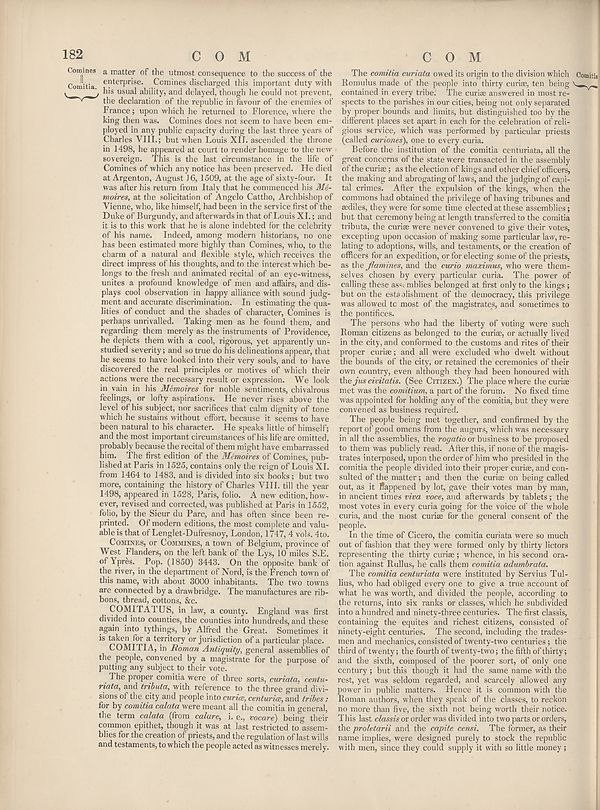
\includegraphics[width=0.85\textwidth]{../scans/page-1102-918dd1676cc2.jpg}
\caption*{Source scan: \texttt{page-1102-918dd1676cc2.jpg}}
\end{figure}

\end{document}
